% FIXME divide this file into files...
\chapter{\RU{Работа с числами с плавающей запятой используя SIMD}
\EN{Working with floatng point numbers using SIMD}}

\label{floating_SIMD}
\index{IEEE 754}
\index{SIMD}
\index{SSE}
\index{SSE2}
\RU{Разумеется, FPU остался в x86-совместимых процессорах в то время, когда ввели расширения \ac{SIMD}}
\EN{Of course, the \ac{FPU} has remained in x86-compatible processors when the \ac{SIMD} extensions were added}.

\EN{The }\ac{SIMD}\RU{-расширения}\EN{ extensions} (SSE2) \RU{позволяют удобнее работать с числами с плавающей 
запятой}\EN{offer an easier way to work with floating-point numbers}.

\RU{Формат чисел остается тот же}\EN{The number format remains the same} (IEEE 754).

\index{x86-64}
\RU{Так что современные компиляторы (включая те, что компилируют под x86-64) 
обычно используют \ac{SIMD}-инструкции вместо FPU-инструкций.}\EN{So, modern compilers (including those generating
for x86-64) usually use \ac{SIMD} instructions instead of FPU ones.}

\RU{Это, можно сказать, хорошая новость, потому что работать с ними легче}
\EN{It can be said that it's good news, because it's easier to work with them}.

\RU{Примеры будем использовать из секции о FPU}\EN{We will reuse here the examples from the FPU section}: \ref{sec:FPU}.

\section{\RU{Простой пример}\EN{Simple example}}

\lstinputlisting{patterns/12_FPU/1_simple/simple.c}

\subsection{x64}

\lstinputlisting[caption=\Optimizing MSVC 2012 x64]{patterns/205_floating_SIMD/simple_MSVC_2012_x64_Ox.asm}

\RU{Собственно, входные значения с плавающей запятой передаются через регистры \XMM{0}-\XMM{3}, 
а остальные --- через стек}\EN{The input floating point values are passed in the \XMM{0}-\XMM{3} registers,
all the rest---via the stack}
\footnote{\href{http://go.yurichev.com/17263}{MSDN: Parameter Passing}}.

$a$ \RU{передается через}\EN{is passed in} \XMM{0}, $b$\EMDASH{}\RU{через}\EN{via} \XMM{1}.
\RU{Но XMM-регистры (как мы уже знаем из секции о \ac{SIMD}: \ref{SIMD_x86}) 128-битные, 
а значения типа \Tdouble --- 64-битные,
так что используется только младшая половина регистра}
\EN{The XMM-registers are 128-bit (as we know from the section about \ac{SIMD}: \ref{SIMD_x86}), 
but the \Tdouble values are 64 bit, so only lower register half is used}.

\index{x86!\Instructions!DIVSD}
\TT{DIVSD} \RU{это SSE-инструкция, означает}\EN{is an SSE-instruction that means} 
``Divide Scalar Double-Precision Floating-Point Values'', 
\RU{и просто делит значение типа \Tdouble на другое, лежащие в младших половинах операндов}\EN{it just divides
one value of type \Tdouble by another, stored in the lower halves of operands}.

\RU{Константы закодированы компилятором в формате IEEE 754}\EN{The constants are encoded by compiler in IEEE 754 format}.

\index{x86!\Instructions!MULSD}
\index{x86!\Instructions!ADDSD}
\TT{MULSD} \AndENRU \TT{ADDSD} \RU{работают так же, только производят умножение и сложение}
\EN{work just as the same, but do multiplication and addition}.

\RU{Результат работы ф-ции типа \Tdouble ф-ция оставляет в регистре \XMM{0}}
\EN{The result of the function's execution in type \Tdouble is left in the in \XMM{0} register}.\\
\\
\RU{Как работает неоптимизирующий MSVC}\EN{That is how non-optimizing MSVC works}:

\lstinputlisting[caption=MSVC 2012 x64]{patterns/205_floating_SIMD/simple_MSVC_2012_x64.asm}

\index{Shadow space}
\RU{Чуть более избыточно}\EN{Slightly redundant}. 
\RU{Входные аргументы сохраняются в}\EN{The input arguments are saved in the} ``shadow space'' (\ref{shadow_space}), 
\RU{причем, только младшие половины регистров, т.е., только 64-битные значения типа \Tdouble}
\EN{but only their lower register halves, i.e., only 64-bit values of type \Tdouble}.\\
\\
\RU{Результат работы компилятора GCC точно такой же}\EN{GCC produces the same code}.

\subsection{x86}

\RU{Я скомпилировал этот пример также и под x86. MSVC 2012 даже генерируя под x86, использует 
SSE2-инструкции:}\EN{I also compiled this example for x86. Despite the fact it's generating for x86, 
MSVC 2012 uses SSE2 instructions:}

\lstinputlisting[caption=\NonOptimizing MSVC 2012 x86]{patterns/205_floating_SIMD/simple_MSVC_2012_x86.asm}

\lstinputlisting[caption=\Optimizing MSVC 2012 x86]{patterns/205_floating_SIMD/simple_MSVC_2012_x86_Ox.asm}

\RU{Код почти такой же, правда есть пара отличий связанных с соглашениями о вызовах:}
\EN{It's almost the same code, however, there are some differences related to calling conventions:}
1) \RU{аргументы передаются не в XMM-регистрах, а через стек, как и прежде, в примерах с FPU (\ref{sec:FPU});}
\EN{the arguments are passed not in XMM registers, but in the stack, like in the FPU examples (\ref{sec:FPU});}
2) \RU{результат работы ф-ции возвращается через \ST{0} --- для этого он через стек
(через локальную переменную \TT{tv}) копируется из XMM-регистра в \ST{0}.}
\EN{the result of the function is returned in \ST{0} --- in order to do so, it's copied
(through local variable \TT{tv}) from one of the XMM registers to \ST{0}.}

\ifdefined\IncludeOlly
\clearpage
\RU{Попробуем соптимизированный пример в}\EN{Let's try the optimized example in} \olly:

\begin{figure}[H]
\centering
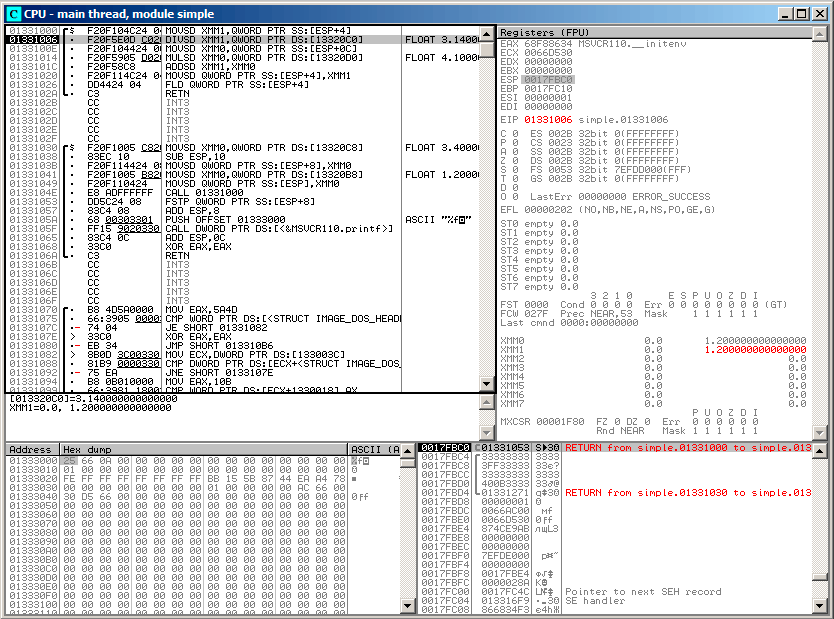
\includegraphics[scale=\FigScale]{patterns/205_floating_SIMD/simple_olly1.png}
\caption{\olly: \TT{MOVSD} \RU{загрузила значение}\EN{loads the value of} $a$ \RU{в}\EN{into} \XMM{1}}
\label{fig:FPU_SIMD_simple_olly1}
\end{figure}

\clearpage
\begin{figure}[H]
\centering
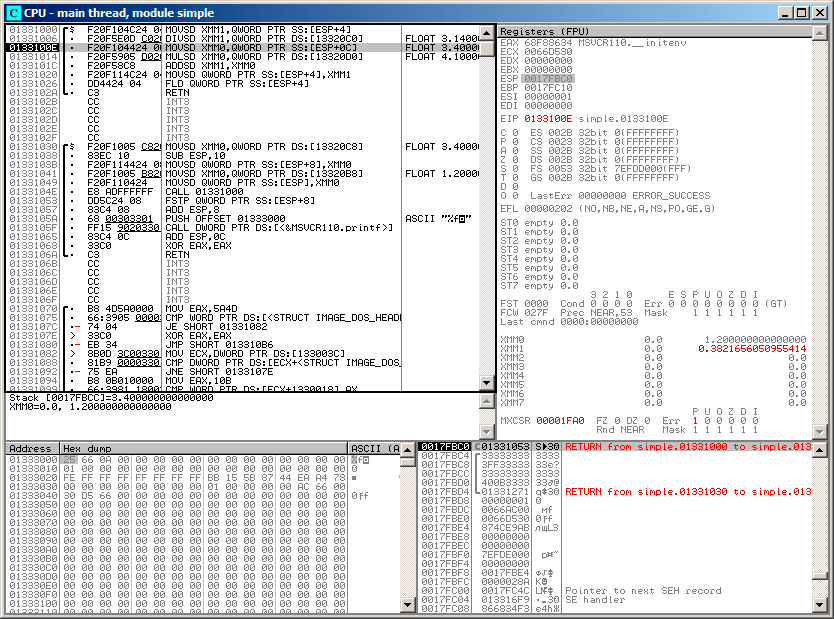
\includegraphics[scale=\FigScale]{patterns/205_floating_SIMD/simple_olly2.png}
\caption{\olly: \TT{DIVSD} \RU{вычислила}\EN{calculated} \gls{quotient} 
\RU{и оставила его в}\EN{and stored it in} \XMM{1}}
\label{fig:FPU_SIMD_simple_olly2}
\end{figure}

\clearpage
\begin{figure}[H]
\centering
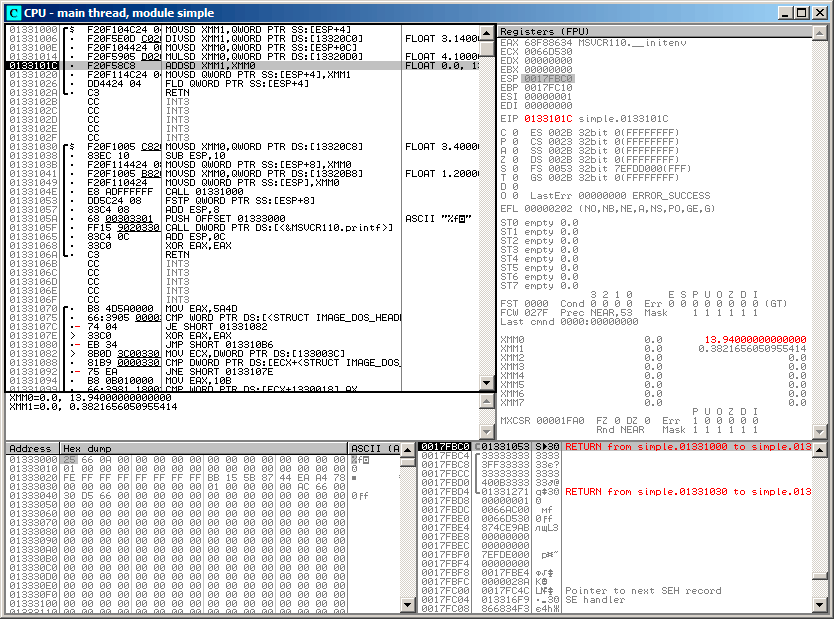
\includegraphics[scale=\FigScale]{patterns/205_floating_SIMD/simple_olly3.png}
\caption{\olly: \TT{MULSD} \RU{вычислила}\EN{calculated} \gls{product} \RU{и оставила его в}\EN{and stored it
in} \XMM{0}}
\label{fig:FPU_SIMD_simple_olly3}
\end{figure}

\clearpage
\begin{figure}[H]
\centering
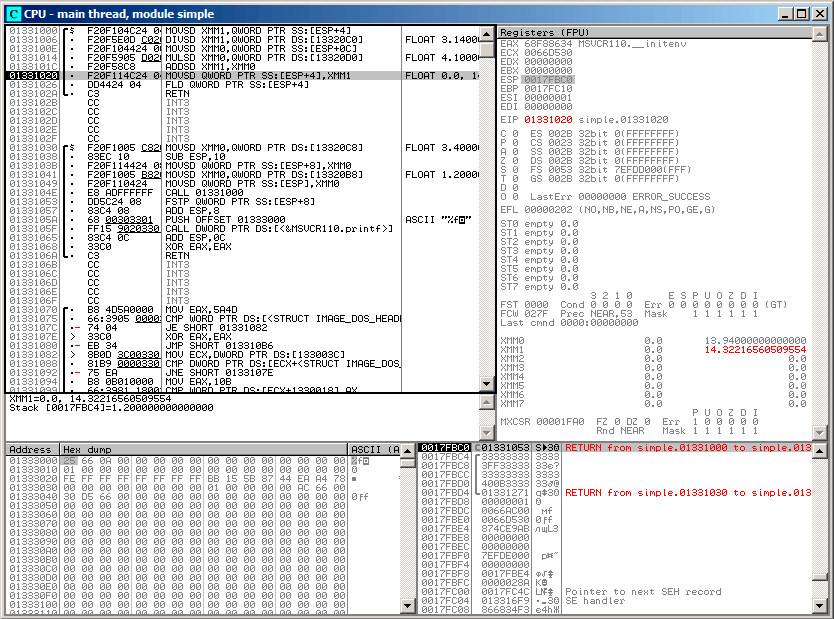
\includegraphics[scale=\FigScale]{patterns/205_floating_SIMD/simple_olly4.png}
\caption{\olly: \TT{ADDSD} \RU{прибавила значение в}\EN{adds value in} \XMM{0} \RU{к}\EN{to} \XMM{1}}
\label{fig:FPU_SIMD_simple_olly4}
\end{figure}

\clearpage
\begin{figure}[H]
\centering
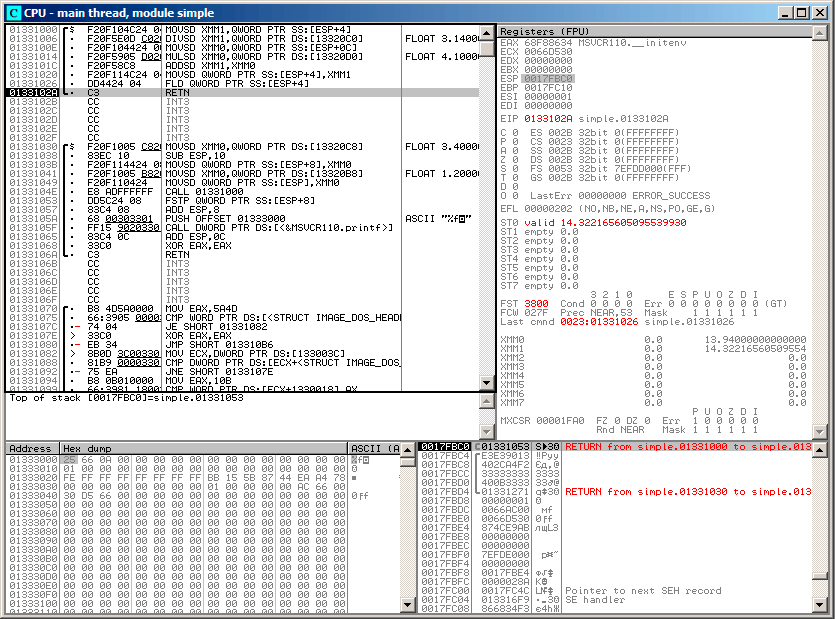
\includegraphics[scale=\FigScale]{patterns/205_floating_SIMD/simple_olly5.png}
\caption{\olly: \FLD \RU{оставляет результат ф-ции в}\EN{left function result in} \ST{0}}
\label{fig:FPU_SIMD_simple_olly5}
\end{figure}

\RU{Видно, что \olly показывает XMM-регистры как пары чисел в формате \Tdouble,
но используется только \IT{младшая} часть.}
\EN{We see that \olly shows the XMM registers as pairs of \Tdouble numbers,
but only the \IT{lower} part is used.}
\RU{Должно быть, \olly показывает их именно так, потому что сейчас исполняются SSE2-инструкции
с суффиксом \TT{-SD}.}
\EN{Apparently, \olly shows them in that format because the SSE2 instructions (suffixed with \TT{-SD}) 
are executed right now.}
\RU{Но конечно же, можно переключить отображение значений в регистрах и посмотреть содержимое
как 4 \Tfloat{}-числа или просто как 16 байт.}
\EN{But of course, it's possible to switch the register format and to see their contents as
4 \Tfloat{}-numbers or just as 16 bytes.}
\fi

\clearpage
\section{\RU{Передача чисел с плавающей запятой в аргументах}\EN{Passing floating point number via arguments}}

\lstinputlisting{patterns/12_FPU/2_passing_floats/pow.c}

\RU{Они передаются в младших половинах регистров}\EN{They are passed in the lower halves
of the} \XMM{0}-\XMM{3}\EN{ registers}.

\lstinputlisting[caption=\Optimizing MSVC 2012 x64]{patterns/205_floating_SIMD/pow_MSVC_2012_x64_Ox.asm}

\index{x86!\Instructions!MOVSD}
\index{x86!\Instructions!MOVSDX}
\RU{Инструкции}\EN{There is no} \TT{MOVSDX} \RU{нет в документации от}\EN{instruction in} 
Intel \cite{Intel} \AndENRU AMD \cite{AMD}\EN{ manuals}, 
\RU{там она называется просто}\EN{there it is called just} \TT{MOVSD}.
\RU{Таким образом, в процессорах x86 две инструкции с одинаковым именем}\EN{So there are two instructions
sharing the same name in x86} (\RU{о второй}\EN{about the other see}: \ref{REP_MOVSx}).
\RU{Возможно, в Microsoft решили избежать
путаницы и переименовали инструкцию в}\EN{Apparently, Microsoft developers wanted to get rid of the mess,
so they renamed it to} \TT{MOVSDX}.
\RU{Она просто загружает значение в младшую половину XMM-регистра}\EN{It just loads a value into
the lower half of a XMM register}.

\RU{Ф-ция }\TT{pow()} \RU{берет аргументы из}\EN{takes arguments from} \XMM{0} \AndENRU \XMM{1}, 
\RU{и возвращает результат в}\EN{and returns result in} \XMM{0}.
\RU{Далее он перекладывается в}\EN{It is then moved to} \RDX \ForENRU \printf. 
\RU{Почему}\EN{Why}? 
\RU{Честно говоря, не знаю, может быть, это потому что}\EN{Honestly speaking, I don't know, maybe because} 
\printf\EMDASH{}\RU{ф-ция с переменным количеством аргументов}\EN{is a variable arguments function}?

\lstinputlisting[caption=\Optimizing GCC 4.4.6 x64]{patterns/205_floating_SIMD/pow_GCC446_x64_O3.s.\LANG}

GCC \RU{работает понятнее}\EN{generates clearer output}. 
\RU{Значение для}\EN{The value for} \printf \RU{передается в}\EN{is passed in} \XMM{0}. 
\RU{Кстати, вот тот случай, когда в}\EN{By the way, here is a case when 1 is written into} \EAX
\ForENRU \printf \RU{записывается 1 --- это значит, что будет передан один аргумент в векторных регистрах, 
так того требует стандарт}\EN{---this means that one argument will be passed in vector registers,
just as the standard requires} \cite{SysVABI}.

\section{\RU{Пример с сравнением}\EN{Comparison example}}

\lstinputlisting{patterns/12_FPU/3_comparison/d_max.c}

\subsection{x64}

\lstinputlisting[caption=\Optimizing MSVC 2012 x64]{patterns/205_floating_SIMD/d_max_MSVC_2012_x64_Ox.asm}

\Optimizing MSVC \RU{генерирует очень понятный код}\EN{generates a code very easy to understand}.

\index{x86!\Instructions!COMISD}
\RU{Инструкция }\TT{COMISD} \RU{это}\EN{is} ``Compare Scalar Ordered Double-Precision Floating-Point 
Values and Set EFLAGS''. \RU{Собственно, это она и делает}\EN{Essentially, that is what it does}.\\
\\
\NonOptimizing MSVC \RU{генерирует более избыточно, но тоже всё понятно}\EN{generates more redundant code,
but it is still not hard to understand}:

\lstinputlisting[caption=MSVC 2012 x64]{patterns/205_floating_SIMD/d_max_MSVC_2012_x64.asm}

\index{x86!\Instructions!MAXSD}
\RU{А вот}\EN{However,} GCC 4.4.6 \RU{дошел в оптимизации дальше и применил инструкцию}
\EN{did more optimizations and used the} \TT{MAXSD} (``Return Maximum Scalar 
Double-Precision Floating-Point Value'')\RU{, которая просто выбирает максимальное значение}\EN{ instruction,
which just choose the maximum value}!

\lstinputlisting[caption=\Optimizing GCC 4.4.6 x64]{patterns/205_floating_SIMD/d_max_GCC446_x64_O3.s}

\clearpage
\subsection{x86}

\RU{Скомпилируем этот пример в MSVC 2012 с включенной оптимизацией:}
\EN{Let's compile this example in MSVC 2012 with optimization turned on:}

\lstinputlisting[caption=\Optimizing MSVC 2012 x86]{patterns/205_floating_SIMD/d_max_MSVC_2012_x86_Ox.asm}

\RU{Всё то же самое, только значения}\EN{Almost the same, but the values of} $a$ \AndENRU $b$ 
\RU{берутся из стека, а результат функции оставляется в}\EN{are taken from the stack and the function result 
is left in} \ST{0}.

\ifdefined\IncludeOlly
\RU{Если загрузить этот пример в}\EN{If we load this example in} \olly, 
\RU{увидим, как инструкция}\EN{we will see how the} \TT{COMISD} \RU{сравнивает значения и устанавливает/сбрасывает
флаги}\EN{instruction compares values and sets/clears the} \CF \AndENRU \PF\EN{ flags}:

\begin{figure}[H]
\centering
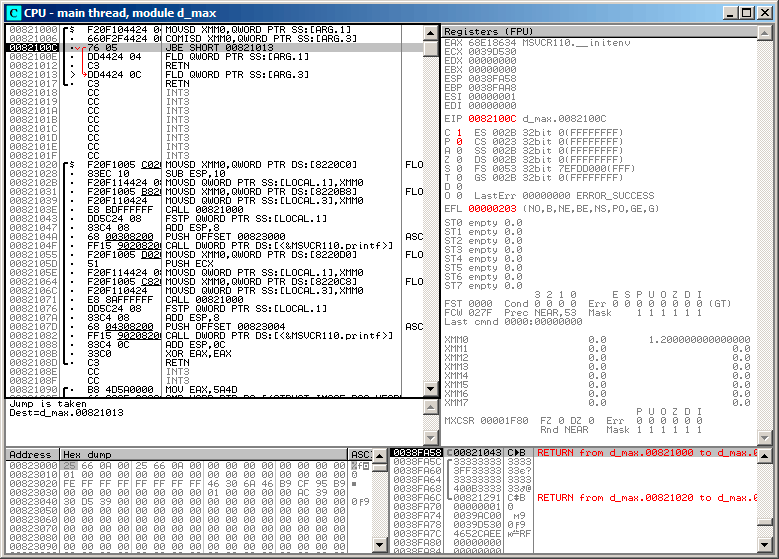
\includegraphics[scale=\FigScale]{patterns/205_floating_SIMD/d_max_olly.png}
\caption{\olly: \TT{COMISD} \RU{изменила флаги}\EN{changed} \CF \AndENRU \PF\EN{ flags}}
\label{fig:FPU_SIMD_d_max_olly}
\end{figure}
\fi

\section{\RU{Вычисление машинного эпсилона}\EN{Calculating machine epsilon}: x64 \AndENRU SIMD}
\label{machine_epsilon_x64_and_SIMD}

\RU{Вернемся к примеру ``вычисление машинного эпсилона'' для \Tdouble \lstref{machine_epsilon_double_c}.}
\EN{Let's revisit the ``calculating machine epsilon'' example for \Tdouble \lstref{machine_epsilon_double_c}.}

\RU{Теперь скомпилируем его для x64}\EN{Now we compile it for x64}:

\lstinputlisting[caption=\Optimizing MSVC 2012 x64]{patterns/205_floating_SIMD/epsilon_double_MSVC_2012_x64_Ox.asm}

\RU{Нет способа прибавить 1 к значению в 128-битном XMM-регистре, так что его нужно в начале поместить в память.}
\EN{There is no way to add 1 to a value in 128-bit XMM register, so it must be placed into memory.}

\RU{Впрочем, есть инструкция ADDSD (\IT{Add Scalar Double-Precision Floating-Point Values}),
которая может прибавить значение к младшей 64-битной части XMM-регистра игнорируя старшую половину,
но наверное MSVC 2012 пока недостаточно хорош для этого}
\EN{There is, however, the ADDSD instruction (\IT{Add Scalar Double-Precision Floating-Point Values}) 
which can add a value to the lowest 64-bit half of a XMM register while ignoring the higher one, 
but MSVC 2012 probably is not that good yet}
\footnote{\RU{В качестве упражнения, вы можете попробовать переработать этот код, чтобы избавиться 
от использования локального стека}\EN{As an exercise, you may try to rework this code to 
eliminate the usage of the local stack}.}.

\RU{Так или иначе, значение затем перезагружается в XMM-регистр и происходит вычитание.}
\EN{Nevertheless, the value is then reloaded to a XMM register and subtraction occurs.}
SUBSD \RU{это}\EN{is} ``Subtract Scalar Double-Precision Floating-Point Values'', 
\RU{т.е., операция производится над младшей 64-битной частью 128-битного XMM-регистра}
\EN{i.e., it operates on the lower 64-bit part of 128-bit XMM register}.
\RU{Результат возвращается в регистре XMM0}\EN{The result is returned in the XMM0 register}.

\section{\RU{И снова пример генератора случайных чисел}\EN{Pseudo-random number generator example revisited}}
\label{FPU_PRNG_SIMD}

\RU{Вернемся к примеру \q{пример генератора случайных чисел} \lstref{FPU_PRNG}.}
\EN{Let's revisit \q{pseudo-random number generator example} example \lstref{FPU_PRNG}.}

\RU{Если скомпилировать это в MSVC 2012, компилятор будет использовать SIMD-инструкции для FPU.}
\EN{If we compile this in MSVC 2012, it will use the SIMD instructions for the FPU.}

\lstinputlisting[caption=\Optimizing MSVC 2012]{patterns/205_floating_SIMD/FPU_PRNG/MSVC2012_Ox_Ob0.asm.\LANG}

% FIXME1 rewrite!
\RU{У всех инструкций суффикс -SS, это означает \q{Scalar Single}.}
\EN{All instructions have the -SS suffix, which stands for \q{Scalar Single}.}
\RU{\q{Scalar} означает что только одно значение хранится в регистре.}
\EN{\q{Scalar} implies that only one value is stored in the register.}
\RU{\q{Single} означает что это тип \Tfloat.}
\EN{\q{Single} stands for \Tfloat data type.}


\section{\RU{Итог}\EN{Summary}}

\RU{Во всех приведенных примерах, в XMM-регистрах используется только младшая половина регистра, там
хранится значение в формате IEEE 754}\EN{Only the lower half of XMM registers is used in all examples here, 
to store number in IEEE 754 format}.

\RU{Собственно, все инструкции с суффиксом}\EN{Essentially, all instructions prefixed by} 
\TT{-SD} (``Scalar Double-Precision'')\EMDASH{}\RU{это инструкции для работы с числами с плавающей 
запятой в формате IEEE 754, 
хранящиеся в младшей 64-битной половине XMM-регистра}\EN{are instructions working with floating point numbers
in IEEE 754 format, stored in the lower 64-bit half of a XMM register}.

\RU{Всё удобнее чем это было в FPU, видимо, сказывается тот факт, что расширения 
SIMD развивались не так хаотично как FPU в прошлом.}
\EN{And it is easier than in the FPU, probably because the SIMD extensions 
were evolved in a less chaotic way than the FPU ones in the past.}
\RU{Стековая модель регистров не используется}\EN{The stack register model is not used}.

\index{x86!\Instructions!ADDSS}
\index{x86!\Instructions!MOVSS}
\index{x86!\Instructions!COMISS}
% TODO: do this!
\RU{Если вы попробуете заменить в этих примерах}\EN{If you would try to replace} \Tdouble \RU{на}\EN{with} \Tfloat
\RU{, то инструкции будут использоваться те же,
только с суффиксом}\EN{in these examples, the same instructions will be used, but prefixed with} \TT{-SS} 
(``Scalar Single-Precision''), \RU{например}\EN{for example}, \TT{MOVSS}, \TT{COMISS}, \TT{ADDSS}, \RU{и т.д.}\EN{etc.}

``Scalar'' \RU{означает что SIMD-регистр будет хранить только одно значение, вместо нескольких}\EN{means that
the SIMD register will contain only one value instead of several}.
\RU{Инструкции, работающие с несколькими значениями в регистре одновременно, имеют ``Packed'' в названии}
\EN{Instructions working with several values in a register simultaneously have ``Packed'' in their name}.

\RU{Нужно также обратить внимание, что SSE2-инструкции работают с 64-битными числами (\Tdouble) в формате IEEE 754,
в то время как внутреннее представление в FPU --- 80-битные числа.}
\EN{Needless to say, the SSE2 instructions work with 64-bit IEEE 754 numbers (\Tdouble),
while the internal representation of the floating-point numbers in FPU is 80-bit numbers.}
\RU{Поэтому ошибок округления (\IT{round-off error}) в FPU может быть меньше чем в SSE2,
как следствие, можно сказать, работа с FPU может даавать более точные результаты вычислений.}
\EN{Hence, the FPU may produce less round-off errors and as a consequence, FPU may give more precise
calculation results.}
